\section{Storyboards}

Dopo la fase di Needfinding abbiamo scelto \textbf{4 task} su cui concentrarci:
\begin{itemize}
    \item \textit{Selezione  Preferenze};
    \item \textit{Ricerca con Filtri};
    \item \textit{Notifica} (in base agli interessi);
    \item \textit{Unione a Visita di Gruppo}.
\end{itemize}

\subsection{Selezione Preferenze}

\begin{figure}[h]
    \centering
    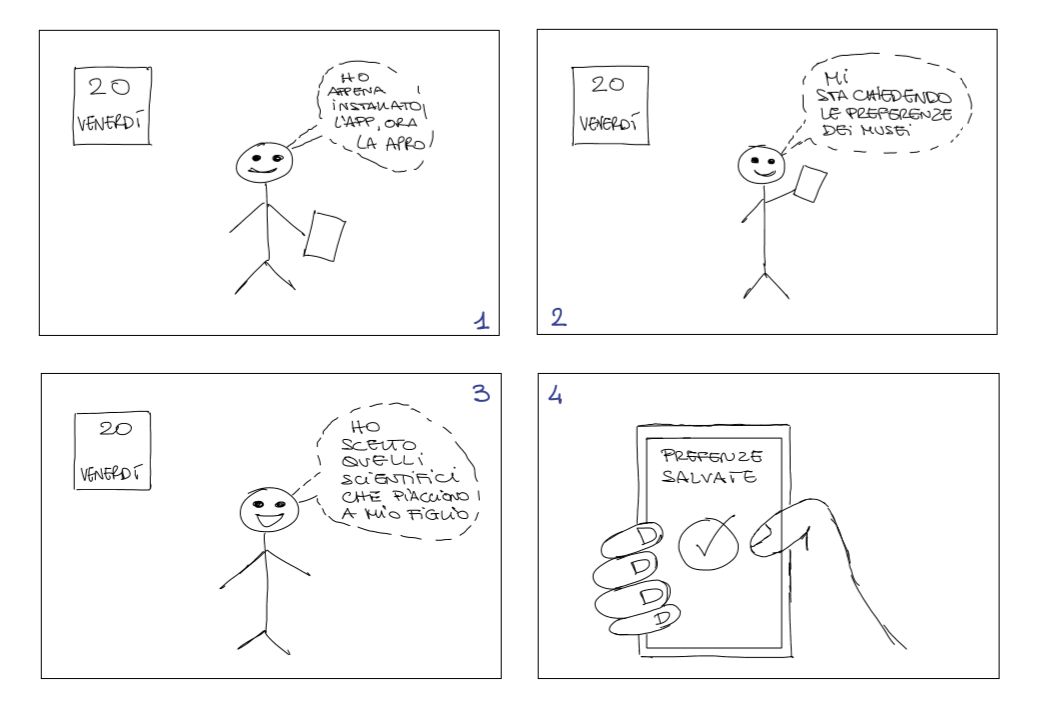
\includegraphics[width=1.0\textwidth]{images/storyboards/Storyboard-1-scelta-preferenze-notitle.png}
\end{figure}

\newpage

\subsection{Ricerca con Filtri}

\begin{figure}[h]
    \centering
    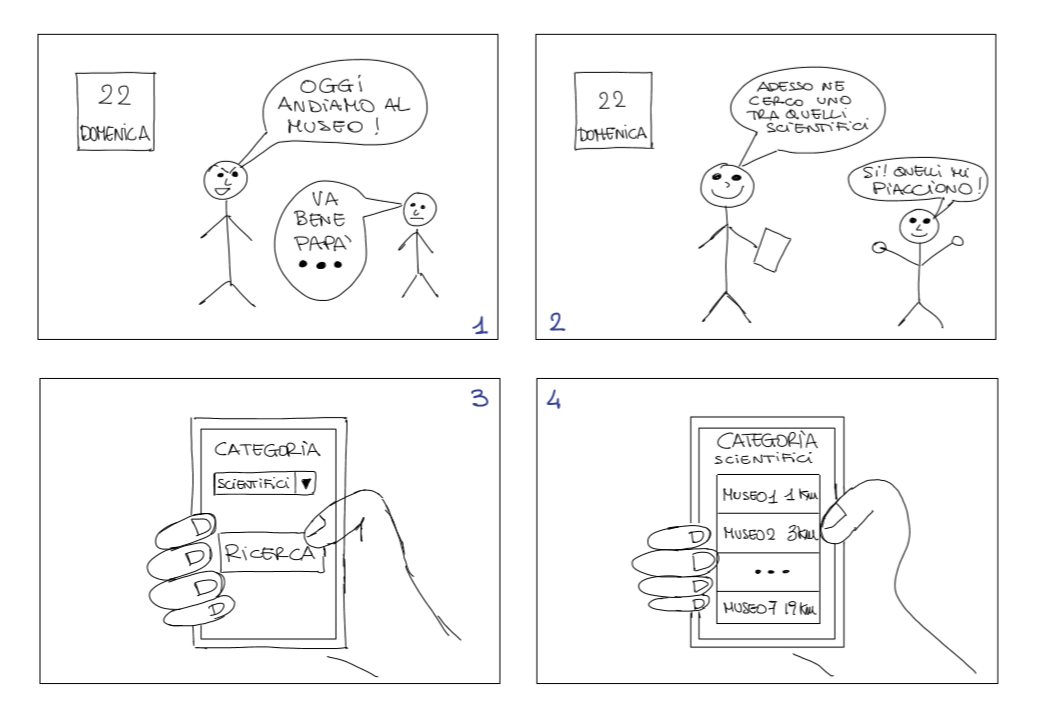
\includegraphics[width=1.0\textwidth]{images/storyboards/Storyboard-2-ricerca-notitle.png}
\end{figure}

\newpage

\subsection{Notifica}

\begin{figure}[h]
    \centering
    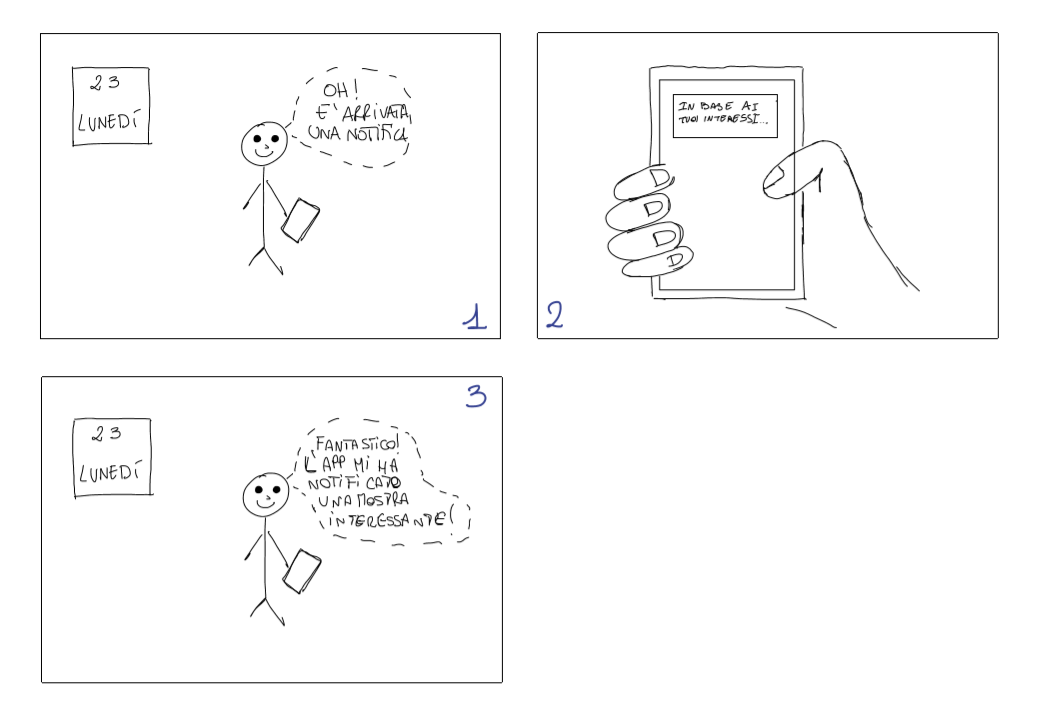
\includegraphics[width=1.0\textwidth]{images/storyboards/Storyboard-3-notifica-notitle.png}
\end{figure}

\newpage

\subsection{Unione a Visita di Gruppo}

\begin{figure}[h]
    \centering
    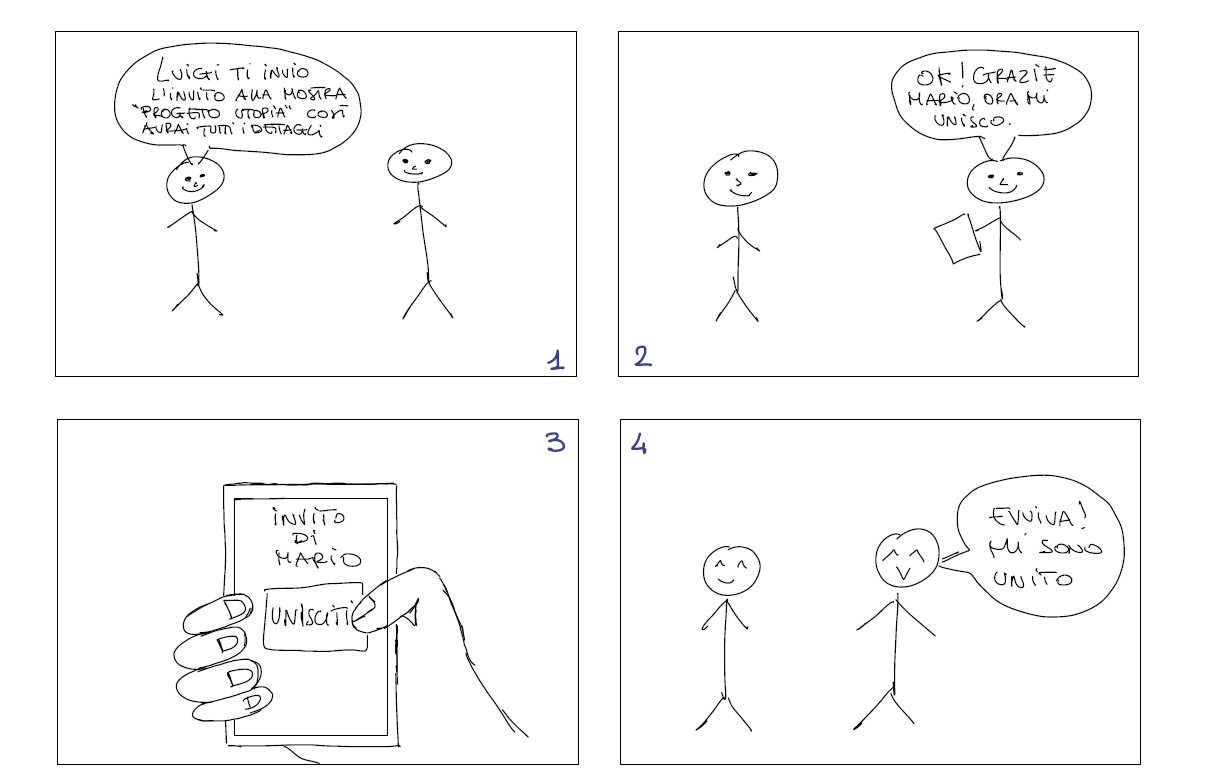
\includegraphics[width=1.0\textwidth]{images/storyboards/Storyboard-4-unione-gruppo-notitle.png}
\end{figure}